%%=============================================================================
%% LaTeX sjabloon voor bachelorproef, HoGent Bedrijf en Organisatie
%% Opleiding Toegepaste Informatica
%%=============================================================================

\documentclass[fleqn,a4paper,12pt]{book}


%%=============================================================================
%% LaTeX sjabloon voor de bachelorproef, HoGent Bedrijf en Organisatie
%% Opleiding toegepaste informatica
%%
%% Structuur en algemene vormgeving. Meestal hoef je hier niets te wijzigen.
%%
%% Vormgeving gebaseerd op "The Legrand Orange Book", version 2.0 (9/2/15)
%% door Mathias Legrand (legrand.mathias@gmail.com) met aanpassingen door
%% Vel (vel@latextemplates.com). Het oorspronkelijke template is te vinden op
%% http://www.LaTeXTemplates.com
%%
%% Aanpassingen voor HoGent toegepaste informatica: 
%%   Bert Van Vreckem <bert.vanvreckem@hogent.be>
%% Licentie: 
%%   CC BY-NC-SA 3.0 (http://creativecommons.org/licenses/by-nc-sa/3.0/)
%%=============================================================================

%%-----------------------------------------------------------------------------
%% Packages
%%-----------------------------------------------------------------------------

\usepackage[top=3cm,bottom=3cm,left=3cm,right=3cm,headsep=10pt,a4paper]{geometry} % Page margins
\usepackage[utf8]{inputenc}  % Accenten gebruiken in tekst (vb. é ipv \'e)
\usepackage{amsfonts}        % AMS math packages: extra wiskundige
\usepackage{amsmath}         %   symbolen (o.a. getallen-
\usepackage{amssymb}         %   verzamelingen N, R, Z, Q, etc.)
\usepackage[english,dutch]{babel}    % Taalinstellingen: woordsplitsingen,
                             %  commando's voor speciale karakters
                             %  ("dutch" voor NL)
\usepackage{iflang}
\usepackage{eurosym}         % Euro-symbool €
\usepackage{geometry}
\usepackage{graphicx}        % Invoegen van tekeningen
\graphicspath{{img/}}       % Specifies the directory where pictures are stored
\usepackage{tikz}            % Required for drawing custom shapes
\usepackage[pdftex,bookmarks=true]{hyperref}
                             % PDF krijgt klikbare links & verwijzingen,
                             %  inhoudstafel
\usepackage{enumitem}        % Customize lists
\setlist{nolistsep}         % Reduce spacing between list items
\usepackage{listings}        % Broncode mooi opmaken
\usepackage{multirow}        % Tekst over verschillende cellen in tabellen
\usepackage{rotating}        % Tabellen en figuren roteren

\usepackage{booktabs}        % Required for nicer horizontal rules in tables

\usepackage{xcolor}          % Required for specifying colors by name
\definecolor{maincolor}{RGB}{0,147,208} % Define the main color used for 
                             % highlighting throughout the book
                             % 0, 147, 208 = officiële kleur HoGent FBO

% Paragraph style: no indent, add space between paragraphs
\setlength{\parindent}{0em}
\setlength{\parskip}{1em}

\usepackage{etoolbox}
\usepackage{titling} % Macros for title, author, etc
\usepackage{lipsum}          % Voor vultekst (lorem ipsum)

%----------------------------------------------------------------------------------------
%	FONTS
%----------------------------------------------------------------------------------------

\usepackage{avant} % Use the Avantgarde font for headings
%\usepackage{times} % Use the Times font for headings
\usepackage{mathptmx} % Use the Adobe Times Roman as the default text font together with math symbols from the Sym­bol, Chancery and Com­puter Modern fonts

\usepackage{microtype} % Slightly tweak font spacing for aesthetics
\usepackage[utf8]{inputenc} % Required for including letters with accents
\usepackage[T1]{fontenc} % Use 8-bit encoding that has 256 glyphs

%------------------------------------------------------------------------------
%	TITLE PAGE
%------------------------------------------------------------------------------

\newcommand{\inserttitlepage}{%
\begin{titlepage}
  \newgeometry{top=2cm,bottom=1.5cm,left=1.5cm,right=1.5cm}
  \begin{center}

    \begingroup
    \rmfamily
    \includegraphics[width=2.5cm]{img/HG-beeldmerk-woordmerk}\\[.5cm]
    Faculteit Bedrijf en Organisatie\\[3cm]
    \titel
    \vfill
    \student\\[3.5cm]
    Scriptie voorgedragen tot het bekomen van de graad van\\professionele bachelor in de toegepaste informatica\\[2cm]
    Promotor:\\
    \promotor\\
    \ifdefempty{\copromotor}{\vspace{2.5cm}}{Co-promotor:\\\copromotor\\[2.5cm]}
    Instelling: \instelling\\[.5cm]
    Academiejaar: \academiejaar\\[.5cm]
    \ifcase \examenperiode \or Eerste \or Tweede \else Derde \fi examenperiode
    \endgroup

  \end{center}
  \restoregeometry
\end{titlepage}
  \emptypage
}

%----------------------------------------------------------------------------------------
%	BIBLIOGRAPHY AND INDEX
%----------------------------------------------------------------------------------------

\usepackage[style=apa,backend=biber]{biblatex}
\usepackage{csquotes}
\DeclareLanguageMapping{dutch}{dutch-apa}
\addbibresource{bachproef-tin.bib} % BibTeX bibliography file
\addbibresource{../voorstel/voorstel.bib}
\defbibheading{bibempty}{}

\usepackage{calc} % For simpler calculation - used for spacing the index letter headings correctly
\usepackage{makeidx} % Required to make an index
\makeindex % Tells LaTeX to create the files required for indexing

%----------------------------------------------------------------------------------------
%	MAIN TABLE OF CONTENTS
%----------------------------------------------------------------------------------------

\usepackage{titletoc} % Required for manipulating the table of contents

\contentsmargin{0cm} % Removes the default margin

% Part text styling
\titlecontents{part}[0cm]
{\addvspace{20pt}\centering\large\bfseries}
{}
{}
{}

% Chapter text styling
\titlecontents{chapter}[1.25cm] % Indentation
{\addvspace{12pt}\large\sffamily\bfseries} % Spacing and font options for chapters
{\color{maincolor!60}\contentslabel[\Large\thecontentslabel]{1.25cm}\color{maincolor}} % Chapter number
{\color{maincolor}}
{\color{maincolor!60}\normalsize\;\titlerule*[.5pc]{.}\;\thecontentspage} % Page number

% Section text styling
\titlecontents{section}[1.25cm] % Indentation
{\addvspace{3pt}\sffamily\bfseries} % Spacing and font options for sections
{\contentslabel[\thecontentslabel]{1.25cm}} % Section number
{}
{\hfill\color{black}\thecontentspage} % Page number
[]

% Subsection text styling
\titlecontents{subsection}[1.25cm] % Indentation
{\addvspace{1pt}\sffamily\small} % Spacing and font options for subsections
{\contentslabel[\thecontentslabel]{1.25cm}} % Subsection number
{}
{\ \titlerule*[.5pc]{.}\;\thecontentspage} % Page number
[]

% List of figures
\titlecontents{figure}[0em]
{\addvspace{-5pt}\sffamily}
{\thecontentslabel\hspace*{1em}}
{}
{\ \titlerule*[.5pc]{.}\;\thecontentspage}
[]

% List of tables
\titlecontents{table}[0em]
{\addvspace{-5pt}\sffamily}
{\thecontentslabel\hspace*{1em}}
{}
{\ \titlerule*[.5pc]{.}\;\thecontentspage}
[]

%----------------------------------------------------------------------------------------
%	MINI TABLE OF CONTENTS IN PART HEADS
%----------------------------------------------------------------------------------------

% Chapter text styling
\titlecontents{lchapter}[0em] % Indenting
{\addvspace{15pt}\large\sffamily\bfseries} % Spacing and font options for chapters
{\color{maincolor}\contentslabel[\Large\thecontentslabel]{1.25cm}\color{maincolor}} % Chapter number
{}
{\color{maincolor}\normalsize\sffamily\bfseries\;\titlerule*[.5pc]{.}\;\thecontentspage} % Page number

% Section text styling
\titlecontents{lsection}[0em] % Indenting
{\sffamily\small} % Spacing and font options for sections
{\contentslabel[\thecontentslabel]{1.25cm}} % Section number
{}
{}

% Subsection text styling
\titlecontents{lsubsection}[.5em] % Indentation
{\normalfont\footnotesize\sffamily} % Font settings
{}
{}
{}

%----------------------------------------------------------------------------------------
%	PAGE HEADERS
%----------------------------------------------------------------------------------------

\usepackage{fancyhdr} % Required for header and footer configuration

\pagestyle{fancy}
\renewcommand{\chaptermark}[1]{\markboth{\sffamily\normalsize\bfseries\chaptername\ \thechapter.\ #1}{}} % Chapter text font settings
\renewcommand{\sectionmark}[1]{\markright{\sffamily\normalsize\thesection\hspace{5pt}#1}{}} % Section text font settings
\fancyhf{} \fancyhead[LE,RO]{\sffamily\normalsize\thepage} % Font setting for the page number in the header
\fancyhead[LO]{\rightmark} % Print the nearest section name on the left side of odd pages
\fancyhead[RE]{\leftmark} % Print the current chapter name on the right side of even pages
\renewcommand{\headrulewidth}{0.5pt} % Width of the rule under the header
\addtolength{\headheight}{2.5pt} % Increase the spacing around the header slightly
\renewcommand{\footrulewidth}{0pt} % Removes the rule in the footer
\fancypagestyle{plain}{\fancyhead{}\renewcommand{\headrulewidth}{0pt}} % Style for when a plain pagestyle is specified

% Removes the header from odd empty pages at the end of chapters
\makeatletter
\renewcommand{\cleardoublepage}{
\clearpage\ifodd\c@page\else
\hbox{}
\vspace*{\fill}
\thispagestyle{empty}
\newpage
\fi}

%----------------------------------------------------------------------------------------
%	THEOREM STYLES
%----------------------------------------------------------------------------------------

\usepackage{amsmath,amsfonts,amssymb,amsthm} % For math equations, theorems, symbols, etc

\newcommand{\intoo}[2]{\mathopen{]}#1\,;#2\mathclose{[}}
\newcommand{\ud}{\mathop{\mathrm{{}d}}\mathopen{}}
\newcommand{\intff}[2]{\mathopen{[}#1\,;#2\mathclose{]}}
\newtheorem{notation}{Notation}[chapter]

% Boxed/framed environments
\newtheoremstyle{maincolornumbox}% % Theorem style name
{0pt}% Space above
{0pt}% Space below
{\normalfont}% % Body font
{}% Indent amount
{\small\bf\sffamily\color{maincolor}}% % Theorem head font
{\;}% Punctuation after theorem head
{0.25em}% Space after theorem head
{\small\sffamily\color{maincolor}\thmname{#1}\nobreakspace\thmnumber{\@ifnotempty{#1}{}\@upn{#2}}% Theorem text (e.g. Theorem 2.1)
\thmnote{\nobreakspace\the\thm@notefont\sffamily\bfseries\color{black}---\nobreakspace#3.}} % Optional theorem note
\renewcommand{\qedsymbol}{$\blacksquare$}% Optional qed square

\newtheoremstyle{blacknumex}% Theorem style name
{5pt}% Space above
{5pt}% Space below
{\normalfont}% Body font
{} % Indent amount
{\small\bf\sffamily}% Theorem head font
{\;}% Punctuation after theorem head
{0.25em}% Space after theorem head
{\small\sffamily{\tiny\ensuremath{\blacksquare}}\nobreakspace\thmname{#1}\nobreakspace\thmnumber{\@ifnotempty{#1}{}\@upn{#2}}% Theorem text (e.g. Theorem 2.1)
\thmnote{\nobreakspace\the\thm@notefont\sffamily\bfseries---\nobreakspace#3.}}% Optional theorem note

\newtheoremstyle{blacknumbox} % Theorem style name
{0pt}% Space above
{0pt}% Space below
{\normalfont}% Body font
{}% Indent amount
{\small\bf\sffamily}% Theorem head font
{\;}% Punctuation after theorem head
{0.25em}% Space after theorem head
{\small\sffamily\thmname{#1}\nobreakspace\thmnumber{\@ifnotempty{#1}{}\@upn{#2}}% Theorem text (e.g. Theorem 2.1)
\thmnote{\nobreakspace\the\thm@notefont\sffamily\bfseries---\nobreakspace#3.}}% Optional theorem note

% Non-boxed/non-framed environments
\newtheoremstyle{maincolornum}% % Theorem style name
{5pt}% Space above
{5pt}% Space below
{\normalfont}% % Body font
{}% Indent amount
{\small\bf\sffamily\color{maincolor}}% % Theorem head font
{\;}% Punctuation after theorem head
{0.25em}% Space after theorem head
{\small\sffamily\color{maincolor}\thmname{#1}\nobreakspace\thmnumber{\@ifnotempty{#1}{}\@upn{#2}}% Theorem text (e.g. Theorem 2.1)
\thmnote{\nobreakspace\the\thm@notefont\sffamily\bfseries\color{black}---\nobreakspace#3.}} % Optional theorem note
\renewcommand{\qedsymbol}{$\blacksquare$}% Optional qed square
\makeatother

% Defines the theorem text style for each type of theorem to one of the three styles above
\newcounter{dummy}
\numberwithin{dummy}{section}
\theoremstyle{maincolornumbox}
\newtheorem{theoremeT}[dummy]{Theorem}
\newtheorem{problem}{Problem}[chapter]
\newtheorem{exerciseT}{Exercise}[chapter]
\theoremstyle{blacknumex}
\newtheorem{exampleT}{Example}[chapter]
\theoremstyle{blacknumbox}
\newtheorem{vocabulary}{Vocabulary}[chapter]
\newtheorem{definitionT}{Definition}[section]
\newtheorem{corollaryT}[dummy]{Corollary}
\theoremstyle{maincolornum}
\newtheorem{proposition}[dummy]{Proposition}

%----------------------------------------------------------------------------------------
%	DEFINITION OF COLORED BOXES
%----------------------------------------------------------------------------------------

\RequirePackage[framemethod=default]{mdframed} % Required for creating the theorem, definition, exercise and corollary boxes

% Theorem box
\newmdenv[skipabove=7pt,
skipbelow=7pt,
backgroundcolor=black!5,
linecolor=maincolor,
innerleftmargin=5pt,
innerrightmargin=5pt,
innertopmargin=5pt,
leftmargin=0cm,
rightmargin=0cm,
innerbottommargin=5pt]{tBox}

% Exercise box
\newmdenv[skipabove=7pt,
skipbelow=7pt,
rightline=false,
leftline=true,
topline=false,
bottomline=false,
backgroundcolor=maincolor!10,
linecolor=maincolor,
innerleftmargin=5pt,
innerrightmargin=5pt,
innertopmargin=5pt,
innerbottommargin=5pt,
leftmargin=0cm,
rightmargin=0cm,
linewidth=4pt]{eBox}

% Definition box
\newmdenv[skipabove=7pt,
skipbelow=7pt,
rightline=false,
leftline=true,
topline=false,
bottomline=false,
linecolor=maincolor,
innerleftmargin=5pt,
innerrightmargin=5pt,
innertopmargin=0pt,
leftmargin=0cm,
rightmargin=0cm,
linewidth=4pt,
innerbottommargin=0pt]{dBox}

% Corollary box
\newmdenv[skipabove=7pt,
skipbelow=7pt,
rightline=false,
leftline=true,
topline=false,
bottomline=false,
linecolor=gray,
backgroundcolor=black!5,
innerleftmargin=5pt,
innerrightmargin=5pt,
innertopmargin=5pt,
leftmargin=0cm,
rightmargin=0cm,
linewidth=4pt,
innerbottommargin=5pt]{cBox}

% Creates an environment for each type of theorem and assigns it a theorem text style from the "Theorem Styles" section above and a colored box from above
\newenvironment{theorem}{\begin{tBox}\begin{theoremeT}}{\end{theoremeT}\end{tBox}}
\newenvironment{exercise}{\begin{eBox}\begin{exerciseT}}{\hfill{\color{maincolor}\tiny\ensuremath{\blacksquare}}\end{exerciseT}\end{eBox}}
\newenvironment{definition}{\begin{dBox}\begin{definitionT}}{\end{definitionT}\end{dBox}}
\newenvironment{example}{\begin{exampleT}}{\hfill{\tiny\ensuremath{\blacksquare}}\end{exampleT}}
\newenvironment{corollary}{\begin{cBox}\begin{corollaryT}}{\end{corollaryT}\end{cBox}}

%----------------------------------------------------------------------------------------
%	REMARK ENVIRONMENT
%----------------------------------------------------------------------------------------

\newenvironment{remark}{\par\vspace{10pt}\small % Vertical white space above the remark and smaller font size
\begin{list}{}{
\leftmargin=35pt % Indentation on the left
\rightmargin=25pt}\item\ignorespaces % Indentation on the right
\makebox[-2.5pt]{\begin{tikzpicture}[overlay]
\node[draw=maincolor!60,line width=1pt,circle,fill=maincolor!25,font=\sffamily\bfseries,inner sep=2pt,outer sep=0pt] at (-15pt,0pt){\textcolor{maincolor}{R}};\end{tikzpicture}} % Orange R in a circle
\advance\baselineskip -1pt}{\end{list}\vskip5pt} % Tighter line spacing and white space after remark

%----------------------------------------------------------------------------------------
%	SECTION NUMBERING IN THE MARGIN
%----------------------------------------------------------------------------------------

\makeatletter
\renewcommand{\@seccntformat}[1]{\llap{\textcolor{maincolor}{\csname the#1\endcsname}\hspace{1em}}}
\renewcommand{\section}{\@startsection{section}{1}{\z@}
{-4ex \@plus -1ex \@minus -.4ex}
{1ex \@plus.2ex }
{\normalfont\large\sffamily\bfseries}}
\renewcommand{\subsection}{\@startsection {subsection}{2}{\z@}
{-3ex \@plus -0.1ex \@minus -.4ex}
{0.5ex \@plus.2ex }
{\normalfont\sffamily\bfseries}}
\renewcommand{\subsubsection}{\@startsection {subsubsection}{3}{\z@}
{-2ex \@plus -0.1ex \@minus -.2ex}
{.2ex \@plus.2ex }
{\normalfont\small\sffamily\bfseries}}
\renewcommand\paragraph{\@startsection{paragraph}{4}{\z@}
{-2ex \@plus-.2ex \@minus .2ex}
{.1ex}
{\normalfont\small\sffamily\bfseries}}

%----------------------------------------------------------------------------------------
%	PART HEADINGS
%----------------------------------------------------------------------------------------

% numbered part in the table of contents
\newcommand{\@mypartnumtocformat}[2]{%
\setlength\fboxsep{0pt}%
\noindent\colorbox{maincolor!20}{\strut\parbox[c][.7cm]{\ecart}{\color{maincolor!70}\Large\sffamily\bfseries\centering#1}}\hskip\esp\colorbox{maincolor!40}{\strut\parbox[c][.7cm]{\linewidth-\ecart-\esp}{\Large\sffamily\centering#2}}}%
%%%%%%%%%%%%%%%%%%%%%%%%%%%%%%%%%%
% unnumbered part in the table of contents
\newcommand{\@myparttocformat}[1]{%
\setlength\fboxsep{0pt}%
\noindent\colorbox{maincolor!40}{\strut\parbox[c][.7cm]{\linewidth}{\Large\sffamily\centering#1}}}%
%%%%%%%%%%%%%%%%%%%%%%%%%%%%%%%%%%
\newlength\esp
\setlength\esp{4pt}
\newlength\ecart
\setlength\ecart{1.2cm-\esp}
\newcommand{\thepartimage}{}%
\newcommand{\partimage}[1]{\renewcommand{\thepartimage}{#1}}%
\def\@part[#1]#2{%
\ifnum \c@secnumdepth >-2\relax%
\refstepcounter{part}%
\addcontentsline{toc}{part}{\texorpdfstring{\protect\@mypartnumtocformat{\thepart}{#1}}{\partname~\thepart\ ---\ #1}}
\else%
\addcontentsline{toc}{part}{\texorpdfstring{\protect\@myparttocformat{#1}}{#1}}%
\fi%
\startcontents%
\markboth{}{}%
{\thispagestyle{empty}%
\begin{tikzpicture}[remember picture,overlay]%
\node at (current page.north west){\begin{tikzpicture}[remember picture,overlay]%
\fill[maincolor!20](0cm,0cm) rectangle (\paperwidth,-\paperheight);
\node[anchor=north] at (4cm,-3.25cm){\color{maincolor!40}\fontsize{220}{100}\sffamily\bfseries\@Roman\c@part};
\node[anchor=south east] at (\paperwidth-1cm,-\paperheight+1cm){\parbox[t][][t]{8.5cm}{
\printcontents{l}{0}{\setcounter{tocdepth}{1}}%
}};
\node[anchor=north east] at (\paperwidth-1.5cm,-3.25cm){\parbox[t][][t]{15cm}{\strut\raggedleft\color{white}\fontsize{30}{30}\sffamily\bfseries#2}};
\end{tikzpicture}};
\end{tikzpicture}}%
\@endpart}
\def\@spart#1{%
\startcontents%
\phantomsection
{\thispagestyle{empty}%
\begin{tikzpicture}[remember picture,overlay]%
\node at (current page.north west){\begin{tikzpicture}[remember picture,overlay]%
\fill[maincolor!20](0cm,0cm) rectangle (\paperwidth,-\paperheight);
\node[anchor=north east] at (\paperwidth-1.5cm,-3.25cm){\parbox[t][][t]{15cm}{\strut\raggedleft\color{white}\fontsize{30}{30}\sffamily\bfseries#1}};
\end{tikzpicture}};
\end{tikzpicture}}
\addcontentsline{toc}{part}{\texorpdfstring{%
\setlength\fboxsep{0pt}%
\noindent\protect\colorbox{maincolor!40}{\strut\protect\parbox[c][.7cm]{\linewidth}{\Large\sffamily\protect\centering #1\quad\mbox{}}}}{#1}}%
\@endpart}
\def\@endpart{\vfil\newpage
\if@twoside
\if@openright
\null
\thispagestyle{empty}%
\newpage
\fi
\fi
\if@tempswa
\twocolumn
\fi}

%----------------------------------------------------------------------------------------
%	CHAPTER HEADINGS
%----------------------------------------------------------------------------------------

% A switch to conditionally include a picture, implemented by  Christian Hupfer
\newif\ifusechapterimage
\usechapterimagetrue
\newcommand{\thechapterimage}{}%
\newcommand{\chapterimage}[1]{\ifusechapterimage\renewcommand{\thechapterimage}{#1}\fi}%
\def\@makechapterhead#1{%
{\parindent \z@ \raggedright \normalfont
\ifnum \c@secnumdepth >\m@ne
\if@mainmatter
\begin{tikzpicture}[remember picture,overlay]
\node at (current page.north west)
{\begin{tikzpicture}[remember picture,overlay]
\node[anchor=north west,inner sep=0pt] at (0,0) {\ifusechapterimage\includegraphics[width=\paperwidth]{\thechapterimage}\fi};
\draw[anchor=west] (\Gm@lmargin,-9cm) node [line width=2pt,rounded corners=15pt,draw=maincolor,fill=white,fill opacity=0.5,inner sep=15pt]{\strut\makebox[22cm]{}};
\draw[anchor=west] (\Gm@lmargin+.3cm,-9cm) node {\huge\sffamily\bfseries\color{black}\thechapter. #1\strut};
\end{tikzpicture}};
\end{tikzpicture}
\else
\begin{tikzpicture}[remember picture,overlay]
\node at (current page.north west)
{\begin{tikzpicture}[remember picture,overlay]
\node[anchor=north west,inner sep=0pt] at (0,0) {\ifusechapterimage\includegraphics[width=\paperwidth]{\thechapterimage}\fi};
\draw[anchor=west] (\Gm@lmargin,-9cm) node [line width=2pt,rounded corners=15pt,draw=maincolor,fill=white,fill opacity=0.5,inner sep=15pt]{\strut\makebox[22cm]{}};
\draw[anchor=west] (\Gm@lmargin+.3cm,-9cm) node {\huge\sffamily\bfseries\color{black}#1\strut};
\end{tikzpicture}};
\end{tikzpicture}
\fi\fi\par\vspace*{270\p@}}}

%-------------------------------------------

\def\@makeschapterhead#1{%
\begin{tikzpicture}[remember picture,overlay]
\node at (current page.north west)
{\begin{tikzpicture}[remember picture,overlay]
\node[anchor=north west,inner sep=0pt] at (0,0) {\ifusechapterimage\includegraphics[width=\paperwidth]{\thechapterimage}\fi};
\draw[anchor=west] (\Gm@lmargin,-9cm) node [line width=2pt,rounded corners=15pt,draw=maincolor,fill=white,fill opacity=0.5,inner sep=15pt]{\strut\makebox[22cm]{}};
\draw[anchor=west] (\Gm@lmargin+.3cm,-9cm) node {\huge\sffamily\bfseries\color{black}#1\strut};
\end{tikzpicture}};
\end{tikzpicture}
\par\vspace*{270\p@}}
\makeatother

%----------------------------------------------------------------------------------------
%	HYPERLINKS IN THE DOCUMENTS
%----------------------------------------------------------------------------------------

\usepackage{hyperref}
\hypersetup{hidelinks,backref=true,pagebackref=true,hyperindex=true,colorlinks=false,breaklinks=true,urlcolor= maincolor,bookmarks=true,bookmarksopen=false,pdftitle={Title},pdfauthor={Author}}
\usepackage{bookmark}
\bookmarksetup{
open,
numbered,
addtohook={%
\ifnum\bookmarkget{level}=0 % chapter
\bookmarksetup{bold}%
\fi
\ifnum\bookmarkget{level}=-1 % part
\bookmarksetup{color=maincolor,bold}%
\fi
}
}

%----------------------------------------------------------------------------------------
%	Java source code
%----------------------------------------------------------------------------------------

% Commando voor invoegen Java-broncodebestanden (dank aan Niels Corneille)
% Gebruik:
%   \codefragment{source/MijnKlasse.java}{Uitleg bij de code}
%
% Je kan dit aanpassen aan de taal die je zelf het meeste gebruikt in je
% bachelorproef.
\newcommand{\codefragment}[2]{ \lstset{%
  language=java,
  breaklines=true,
  float=th,
  caption={#2},
  basicstyle=\scriptsize,
  frame=single,
  extendedchars=\true
}
\lstinputlisting{#1}}

% Leeg blad
\newcommand{\emptypage}{%
\newpage
\thispagestyle{empty}
\mbox{}
\newpage
}


%%---------- Documenteigenschappen --------------------------------------------
%% TODO: Vul dit aan met je eigen info:

% Je eigen naam
\newcommand{\student}{Thibault Gobert}

% De naam van je promotor (lector van de opleiding)
\newcommand{\promotor}{Harm De Weirdt}

% De naam van je co-promotor. Als je promotor ook je opdrachtgever is en je
% dus ook inhoudelijk begeleidt (en enkel dan!), mag je dit leeg laten.
\newcommand{\copromotor}{}

% Indien je bachelorproef in opdracht van/in samenwerking met een bedrijf of
% externe organisatie geschreven is, geef je hier de naam. Zoniet laat je dit
% zoals het is.
\newcommand{\instelling}{---}

% De titel van het rapport/bachelorproef
\newcommand{\titel}{Redux uitbreiding gebaseerd op Redux-store}

% Datum van indienen (gebruik telkens de deadline, ook al geef je eerder af)
\newcommand{\datum}{28 mei 2018}

% Academiejaar
\newcommand{\academiejaar}{2017-2018}

% Examenperiode
%  - 1e semester = 1e examenperiode => 1
%  - 2e semester = 2e examenperiode => 2
%  - tweede zit  = 3e examenperiode => 3
\newcommand{\examenperiode}{2}

%%=============================================================================
%% Inhoud document
%%=============================================================================

\begin{document}

%---------- Taalselectie ------------------------------------------------------
% Als je je bachelorproef in het Engels schrijft, haal dan onderstaande regel
% uit commentaar. Let op: de tekst op de voorkaft blijft in het Nederlands, en
% dat is ook de bedoeling!

%\selectlanguage{english}

%---------- Titelblad ---------------------------------------------------------
\inserttitlepage

%---------- Samenvatting, voorwoord -------------------------------------------
\usechapterimagefalse
%%=============================================================================
%% Voorwoord
%%=============================================================================

\chapter*{Woord vooraf}
\label{ch:voorwoord}

%% TODO:
%% Het voorwoord is het enige deel van de bachelorproef waar je vanuit je
%% eigen standpunt (``ik-vorm'') mag schrijven. Je kan hier bv. motiveren
%% waarom jij het onderwerp wil bespreken.
%% Vergeet ook niet te bedanken wie je geholpen/gesteund/... heeft

Op mijn stage werd ik het eerst geconfronteerd met dit probleem. Ik moest daar namelijk de integratie voorzien van een react-redux project (Scratch). De reden waarom ik dit project ook heb gekozen is omdat ik dit project het beste ken en daardoor zo weinig mogelijk tijd zou verliezen door mij te verdiepen in een ander project. Nu scratch overgeschakeld is op JavaScript voor hun graphical user interface, wordt het zeer interessant om een makkelijke manier te voorzien om dit project te integreren. Zeker voor een bedrijf zoals CodeFever, waar ik stage heb gedaan. Zij voorzien namelijk programmeerlessen voor kinderen, dus het zou zeer handig zijn moesten zij een ingebouwde versie van Scratch hebben. 

Wat mij dan verontruste was dat er quasi niets van documentatie hierover te vinden was online. Dit vond ik zeer raar, omdat het net zo belangrijk is om dit te kunnen doen. Dit zorgde er ook voor dat ik een oplossing voor dit probleem wou vinden. 

Verder wil ik nog Harm De Weirdt bedanken voor de begeleiding alsook Simon De Gheselle om mijn co-promotor te zijn. Finaal bedank ik ook de Hogeschool Gent om het mogelijk te maken deze scriptie te schrijven.
%%=============================================================================
%% Samenvatting
%%=============================================================================

% TODO: De "abstract" of samenvatting is een kernachtige (~ 1 blz. voor een
% thesis) synthese van het document.
%
% Deze aspecten moeten zeker aan bod komen:
% - Context: waarom is dit werk belangrijk?
% - Nood: waarom moest dit onderzocht worden?
% - Taak: wat heb je precies gedaan?
% - Object: wat staat in dit document geschreven?
% - Resultaat: wat was het resultaat?
% - Conclusie: wat is/zijn de belangrijkste conclusie(s)?
% - Perspectief: blijven er nog vragen open die in de toekomst nog kunnen
%    onderzocht worden? Wat is een mogelijk vervolg voor jouw onderzoek?
%
% LET OP! Een samenvatting is GEEN voorwoord!

%%---------- Nederlandse samenvatting -----------------------------------------
%
% TODO: Als je je bachelorproef in het Engels schrijft, moet je eerst een
% Nederlandse samenvatting invoegen. Haal daarvoor onderstaande code uit
% commentaar.
% Wie zijn bachelorproef in het Nederlands schrijft, kan dit negeren, de inhoud
% wordt niet in het document ingevoegd.

\IfLanguageName{english}{%
\selectlanguage{dutch}
\chapter*{Samenvatting}
\lipsum[1-4]
\selectlanguage{english}
}{}

%%---------- Samenvatting -----------------------------------------------------
% De samenvatting in de hoofdtaal van het document

\chapter*{\IfLanguageName{dutch}{Samenvatting}{Abstract}}

In dit onderzoek worden twee React-Redux projecten opgesteld. React maakt gebruik van JavaScript voor het bouwen van user interfaces, waar Redux een concept is voor data storage en communicatie binnen de applicatie. Redux functioneert als een state container voor JavaScript apps. Een store is een concept van Redux die de hele state tree van de applicatie vasthoudt.

Het probleem situeert zich in het samenvoegen van twee React-Redux projecten. Deze hebben beide een store die de overeenkomstige state tree bevat. Er kan dus niet rechtstreeks een component geïmporteerd worden van het ene project naar het andere, omdat het daar geen bekende state zal hebben en er zo geen acties op kunnen uitgevoerd worden.

Tot dusver is er nog geen bekende manier om de combinatie van een root reducer ongedaan te maken en opnieuw te combineren met de reducers van alle projecten samen. Dit zou wel nodig zijn om een lineaire state tree te behouden en geen geneste state tree met meerdere gecombineerde reducers.

Om het probleem te reproduceren worden dus twee React-Redux projecten opgesteld. Het eerste project is het hoofdproject  met een basis inlog functionaliteit. Het tweede project is een fork van het bestaande open source project van Scratch. Om beide projecten met elkaar te laten communiceren zal het tweede project gepubliceerd worden op npm onder een eigen registry. Dit zorgt ervoor dat het project geïnstalleerd kan worden als dependency in het eerste project. Op deze manier kan een component snel geïmporteerd worden. 

De bedoeling van dit onderzoek is om een manier te vinden waarbij geen extra aanpassingen moeten gebeuren aan het eerste project, maar enkel een geupdatete versie van het tweede project moet gepublished worden op npm. Er wordt gezocht naar een manier om een lineaire state tree te hebben voor alle reducers samen.
Deze manier zal verkregen worden door een extensie te schrijven op Redux die de mogelijheid biedt om de functionaliteit van het tweede project te gebruiken in het eerste project. 


%---------- Inhoudstafel ------------------------------------------------------
\pagestyle{empty} % No headers
\tableofcontents % Print the table of contents itself
\cleardoublepage % Forces the first chapter to start on an odd page so it's on the right
\pagestyle{fancy} % Print headers again

%---------- Lijst figuren, afkortingen, ... -----------------------------------

% Indien gewenst kan je hier een lijst van figuren/tabellen opgeven. Geef in
% dat geval je figuren/tabellen altijd een korte beschrijving:
%
%  \caption[korte beschrijving]{uitgebreide beschrijving}

\listoffigures
\listoftables

% Als je een lijst van afkortingen of termen wil toevoegen, dan hoort die
% hier thuis. Gebruik bijvoorbeeld de ``glossaries'' package.
% https://www.sharelatex.com/learn/Glossaries

%%---------- Kern -------------------------------------------------------------

%%=============================================================================
%% Inleiding
%%=============================================================================

\chapter*{Inleiding}
\label{ch:inleiding}

\section{Context}
\label{sec:context}

Zoals eerder vermeld, wordt gebruik gemaakt van twee React-Redux projecten. React is een JavaScript library voor het bouwen van user interfaces. React werkt met components. In de component schrijf je de gewenste code die moet gerenderd worden. Een component ontvangt parameters, genaamd \textit{props} en retourneert hiërarchische views die getoond worden door de render methode. Elke component kan onafhankelijk functioneren, wat het dus mogelijk maakt om verschillende components in een andere component in te laden. \autocite{React01} 

Redux is een state container voor JavaScript apps. Redux kan dus gebruikt worden samen met React of andere view libraries. 
In Redux zijn er een aantal basis begrippen die moeten uitgelegd worden voor de verdere voortgang voor dit onderzoek, zoals: actions, reducers, store en containers. Deze begrippen vormen eigenlijk de omkadering van Redux. \autocite{Redux02}

De Redux architectuur heeft een unidirectionele data, dit wil zeggen dat de data steeds dezelfde richting/flow aanneemt. Dit zorgt er voor dat de logica van de applicatie voorspelbaar wordt.  

Een container component is een component die verantwoordelijk is voor het verkrijgen van data. Een container component gaat subscriben op de store, om zo een deel van de Redux state tree te kunnen lezen. Het gaat eigenlijk de nodige delen van de data nemen en doorgeven als \textit{props}. Een container component is ook verantwoordelijk voor het dispatchen van actions die veranderingen maken aan de state van de applicatie. 

Deze actions zijn payloads van informatie die data verzenden van de applicatie naar de store. Actions zijn tevens de enige soort van informatie voor de store. Het zijn JavaScript objecten die een \textit{type} property moeten hebben om aan te duiden welke actie uitgevoerd wordt. Deze types zijn string constanten die in een aparte module worden opgeslaan. 

Als er dan gekeken wordt naar de data flow dan worden er eerst actions gedispatched naar de store. De store zal dan de corresponderende reducer aanroepen met twee argumenten, namelijk de huidige state en de action. Hierna zal de root reducer de output van meerdere reducers combineren in een single state tree. Daarna gaat de Redux store de volledige state tree die geretourneerd werd door de root reducer gaan opslaan. Hier kan de container dan data uit lezen en doorgeven aan een presentationele component.

Reducers specificeren hoe de applicatie zijn state verandert ten gevolge van de actions die verzonden zijn naar de store. Actions beschrijven alleen maar het feit dat er iets gebeurd is, ze beschrijven niet hoe de applicatie zijn state verandert.
Vooraleer er kan gezegd worden hoe een reducer dit doet, moet worden uitgelegd wat een pure functie is. Een pure functie is een functie die met dezelfde input altijd dezelfde output produceert. \autocite{Pure01}

Een reducer is een pure functie die de vorige state en een actie neemt en daaruit de nieuwe state retourneert. Het is belangrijk dat de reducer puur blijft, een aantal zaken zijn een no-go zoals API-calls en niet-pure functies aanroepen. De uitkomst moet voorspelbaar blijven. Redux roept de reducer aan met een \textit{undefined} state voor de eerste keer. Daar moet de initial state van de applicatie worden ingesteld. \autocite{Redux02}

Actions representeren het feit dat er iets gebeurd is en reducers updaten de state aan de hand van deze actions. De store is een object die deze zaken samenbrengt. Deze store heeft een aantal verantwoordelijkheden: 
\begin{itemize}
	\item vasthouden van de state van de applicatie
	\item toegang geven tot de state van de applicatie
	\item toelaten om de state te updaten
	\item registreren van listeners
\end{itemize}
Het laatste punt laat toe om een callback te registreren die de redux store zal aanroepen elke keer een action wordt gedispatched. Op deze manier kan de UI van de applicatie upgedate worden naargelang de state van de applicatie. 



\section{Probleemstelling}
\label{sec:probleemstelling}

Het probleem ligt in het gebruiken van components uit een tweede React-Redux project. Door het importeren van een container component in het eerste project worden de actions die gedispatched worden door die component niet herkend in de store. Deze zitten namelijk in de store van het tweede project. Door de reducers te combineren van beide projecten in een grote root reducer wordt dit probleem opgelost. Dit is zo omdat de store dan de corresponderende reducer kan aanroepen naargelang de action die gedispatched wordt. Het probleem hierbij is dat de reducers van het tweede project gekopieerd zouden moeten worden in de root reducer van het eerste project. Dit resulteert in onstabiele code wanneer er reducers toegevoegd en/of verwijderd worden in het tweede project. Dit onderzoek heeft een meerwaarde voor bedrijven/personen die een React-Redux project hebben en functionaliteit (componenten) willen gebruiken uit een bestaande React-Redux repository. 


\section{Onderzoeksvraag}
\label{sec:onderzoeksvraag}

Onderzoeksvraag:
\begin{itemize}
	\item Hoe kan een tweede react-redux project geïntegreerd worden in een ander react-redux project?

\end{itemize}

Deelonderzoeksvraag:
\begin{itemize}
	\item Hoe kunnen twee root reducers met elkaar gecombineerd worden?
\end{itemize}

\section{Onderzoeksdoelstelling}
\label{sec:onderzoeksdoelstelling}
Het beoogde resultaat van de bachelorproef is om een minimaal aantal lines of code en onderhoud te hebben. Idealiter is dit een aangepaste versie van de functie \textit{combineReducers} waarbij er twee root reducers worden gecombineerd met elkaar zonder nesting te veroorzaken. Verder is het vooral belangrijk dat de functionaliteit behouden wordt van beide projecten.

\section{Opzet van deze bachelorproef}
\label{sec:opzet-bachelorproef}

% Het is gebruikelijk aan het einde van de inleiding een overzicht te
% geven van de opbouw van de rest van de tekst. Deze sectie bevat al een aanzet
% die je kan aanvullen/aanpassen in functie van je eigen tekst.

De rest van deze bachelorproef is als volgt opgebouwd:

In Hoofdstuk~\ref{ch:stand-van-zaken} wordt een overzicht gegeven van de stand van zaken binnen het onderzoeksdomein, op basis van een literatuurstudie.

In Hoofdstuk~\ref{ch:methodologie} wordt de methodologie toegelicht en worden de gebruikte onderzoekstechnieken besproken om een antwoord te kunnen formuleren op de onderzoeksvragen.

% TODO: Vul hier aan voor je eigen hoofstukken, één of twee zinnen per hoofdstuk

In Hoofdstuk~\ref{ch:conclusie}, tenslotte, wordt de conclusie gegeven en een antwoord geformuleerd op de onderzoeksvraag. Daarbij wordt ook een aanzet gegeven voor toekomstig onderzoek binnen dit domein.


\chapter{Literatuurstudie}
\label{ch:stand-van-zaken}

% Tip: Begin elk hoofdstuk met een paragraaf inleiding die beschrijft hoe
% dit hoofdstuk past binnen het geheel van de bachelorproef. Geef in het
% bijzonder aan wat de link is met het vorige en volgende hoofdstuk.

% Pas na deze inleidende paragraaf komt de eerste sectiehoofding.
\paragraph{Inleiding}
Zoals eerder vermeld wordt er gebruik gemaakt van twee React-Redux projecten. In dit hoofdstuk wordt meer informatie gegeven omtrent de achtergrond van deze projecten en wat er nodig is om deze met elkaar te laten communiceren. React bestaat uit JavaScript en om een hogere compatibiliteit te verkrijgen wordt JSX gebruikt omdat deze HTML syntax kan laten bestaan met JavaScript code. Conceptueel bestaat React uit components, elk deel functionaliteit zal een component zijn. Dit voorhoogt ook de herbruikbaarheid van de code. Deze components hebben een lifecycle die doorlopen wordt met een initialisatie, een mount fase, een update en een unmount fase. Daarnaast wordt gebruik gemaakt van Redux om makkelijk de state van de applicatie te beheren. In grote projecten kan het soms moeilijk zijn om te weten wat er waar precies aan het gebeuren is. Om deze state te beheren wordt er hier ook gebruik gemaakt van een bepaalde flow. Container components gaan meestal zorgen voor de connectie tussen React en Redux. 

\section{React}
Volgens \autocite{React01} is React een JavaScript library om user interfaces te bouwen. React is component-based. Een component implementeert een \textit{render} methode die data als input neemt en een view retourneert. Om dit te doen wordt JSX gebruikt. Er kunnen simpele views gemaakt worden voor elke state van de applicatie en React zal deze updaten en de juiste componenten renderen wanneer de data verandert.

\subsection{JSX}
JSX is een XML/HTML-achtige syntax gebruikt door React die ECMAScript uitbreidt zodat XML/HTML-achtige text kan bestaan met JavaScript/React code. Deze syntax is bedoeld om gebruikt te worden door preprocessoren (zoals Babel) om HTML text gevonden in JavaScript files om te zetten in standaard JavaScript objecten. Dit wil dus zeggen dat je door JSX te gebruiken HTML structuren en JavaScript code kan schrijven in dezelfde file, Babel zal dan alle uitdrukkingen vertalen naar JavaScript code. Waar vroeger dus JavaScript code in HTML werd geplaatst, laat JSX het toe om HTML in JavaScript te plaatsen.
\autocite{jsx}

\subsection{Components}
Een enkele view van een user interface is opgedeeld in een aantal stukken, in een aantal components. De start component bevat een tree, die tree kan opgedeeld worden in een aantal sub-components. Deze kunnen dan weer opgedeeld worden in nog meer sub-components. Dit kan dus resulteren in een complexe tree met verschillende React components. Er zijn echter ook nog verschillende soorten components, namelijk \textit{simple} en \textit{stateful}. 
\autocite{jsx}

\paragraph{Simple component}
React components implementeren de \textit{render} methode, ze retourneren wat er moet afgebeeld worden. Daarvoor wordt het eerder aangekaarte JSX gebruikt. Input data die doorgegeven is aan de component kan worden opgeroepen door de \textit{props} aan te spreken van deze component. Sidenote: JSX is optioneel, het gewenste resultaat kan ook bereikt worden door JavaScript code alleen. JSX maakt het wel overzichtelijker om de props aan te spreken.  
\autocite{React01}

\paragraph{Stateful component}
In toevoeging met data als input nemen (via \textit{props}), kan een component zijn interne state aanspreken om daar data uit te halen. Wanneer de data uit de state van een component verandert, wordt de render methode opnieuw aangeroepen zodat de juiste data getoond wordt.
\autocite{React01}




\subsection{React lifecycle}
Met React is het mogelijk om components te creëren door de voorziene methode van React te gebruiken. Deze methode verwacht een \textit{render} methode en zal een lifecycle triggeren, de lifecycle van een component. 
Deze lifecycle kan onderverdeeld worden in 4 grote fasen zoals beschreven in figuur 1.1 en 1.2:
\newline
\begin{itemize}
	\item initialisatie
	\item mounten
	\item updaten
	\item unmounten
\end{itemize}
\begin{figure}
	\begin{center}
		\caption{De initialisatie en de mounting fase van de React lifecycle. Verkregen van \textcite{reactlifecycle}.}
		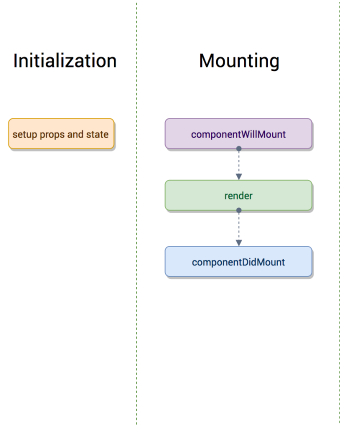
\includegraphics[width=8cm]{img/react-lifecycle1}\\[0.5cm]
	\end{center}
\end{figure}

\begin{figure}
	\begin{center}
		\caption{De update en de unmount fase van de React lifecycle. Verkregen van \textcite{reactlifecycle}.}
		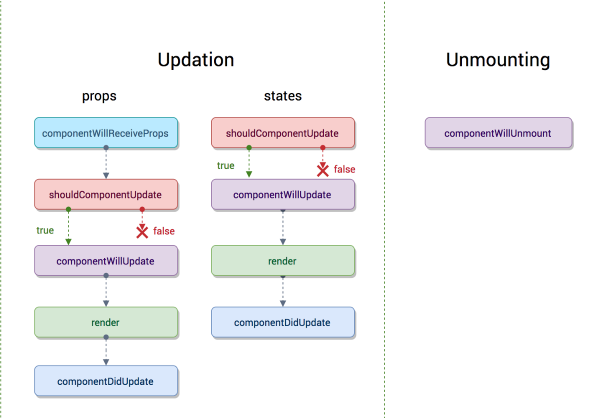
\includegraphics[width=15cm]{img/react-lifecycle2}\\[0.5cm]
	\end{center}
\end{figure}

\paragraph{Initialisatie}
In deze fase worden de initiële state en de default props ingesteld. De initiële state wordt in de constructor ingesteld, deze kan later altijd veranderd worden door de \textit{setState} methode. \textit{defaultProps} is een property van \textit{Component} die overschreven kan worden met nieuwe waarden voor de props. 

\paragraph{Mounten}
In de tweede fase zijn er een aantal \textit{hook} methodes die aangeroepen kunnen worden voor het mounten en na het mounten. Een hook methode is een methode waar je kan inpikken in de lifecycle en bestaande code kan veranderen of verbeteren naar eigen noden. 

Al de dingen die moeten gebeuren voor een component gaat mounten, moeten gedefinieerd zijn in de \textit{componentWillMount}. Deze methode wordt een keer per lifecycle uitgevoerd voor de eerste \textit{render}. 

Render zal de component mounten in de browser. Het is een pure methode, dus het geeft altijd dezelfde output gegeven dezelfde input. 

Na deze eerste render, wordt de methode \textit{componentDidMount} aangeroepen. Deze methode wordt opnieuw een keer per lifecycle uitgevoerd. 

\paragraph{Updaten}
Deze derde fase start wanneer de React component succesvol gerenderd is op de browser. De component kan nu geüpdatet worden op twee manieren: het verzenden van nieuwe props of het updaten van de state. 

Wanneer de component nieuwe props ontvangt of de state is geüpdatet, wordt in de methode \textit{shouldComponentUpdate} gevraagd of er een re-render moet gebeuren of niet. Deze methode retourneert dus een boolean en zal standaard re-renderen tenzij anders beschreven. Het is dus mogelijk om enkel een re-render uit te voeren als de props veranderen. Deze hook methode wordt vooral gebruikt als renderen een zware methode is. Dan is het niet voordelig om altijd alles opnieuw te renderen.

Als de uitkomst van deze methode true is, dan zal de component updaten en wordt de hook methode \textit{componentWillUpdate} opgeroepen. In deze methode worden de nodige voorbereidingen gedaan voor de volgende render, gelijkaardig als \textit{componentWillMount}. Hierna wordt de component dus opnieuw gerenderd. 

Wanneer dit succesvol is dan zal \textit{componentDidUpdate} de third party libraries updaten en reloaden. 

Wanneer echter de props veranderen en het is niet de eerste render dan zal in \textit{componentWillReceiveProps} de state en de props opnieuw gesynchroniseerd worden met elkaar. 

\paragraph{Unmounten}
In de laatste fase is de component niet meer nodig en zal deze via \textit{componentWillUnmount} verwijderd worden. Hier kan er dan een cleanup gebeuren wat betreft user details en authorization tokens.
\autocite{reactlifecycle}
\autocite{reactlifecycle2}


\section{Redux}
De requirements voor JavaScript single-page applicaties worden meer en meer gecompliceerd. De code moet veel meer state beheren dan vroeger. Deze state kan server responses en gecachete data, maar ook lokaal gecreëerde data die nog niet naar de server is doorgestuurd bevatten. Deze steeds veranderende state beheren is moeilijk. Als een model een ander model kan updaten, waar een view dan een ander model kan updaten, die een nieuw model gaat updaten, die op zijn beurt ook nog eens een view kan updaten. Op een gegeven moment wordt het niet meer duidelijk wat er gebeurt in de applicatie. Wanneer een systeem ondoorzichtig en niet-deterministisch is, wordt het moeilijk om bugs te reproduceren of om nieuwe features toe te voegen. Deze complexiteit is moeilijk om mee om te gaan omdat er twee concepten in verwikkeld worden die moeilijk vatbaar zijn: mutatie en asynchroniteit. Beide kunnen apart heel handig zijn, maar samen kan dit voor heel wat problemen zorgen.

Door stateful components die elkaar aanroepen verhoogt de complexiteit om de state te beheren. Om tegen te gaan dat de controle verloren gaat over wanneer, hoe en waarom de state geüpdatet wordt, kan redux geïntroduceerd worden als oplossing om de state te managen. Redux zal proberen om de veranderingen op de state voorspelbaar te maken door bepaalde restricties op te leggen omtrent het updaten van de state. Deze restricties staan beschreven in de \textit{drie principes} van Redux.

\subsection{Drie principes}

\paragraph{Een enkele source}  
De state van de hele applicatie zit in een object tree in een enkele \textit{store}. Een enkele state maakt het makkelijker om te debuggen of om de applicatie te inspecteren. Sommige functionaliteit kan snel geïmplementeerd worden hierdoor, zoals een undo/redo waar dan geswitched kan worden tussen een vorige en een volgende state van de applicatie. Dit kan dus enkel wanneer de hele state van de applicatie is opgeslagen in de object tree.

\paragraph{State is read-only}
De enige manier om een state te veranderen is door het verzenden van een \textit{action}, dit is een object dat beschrijft wat er gebeurt. Dit zorgt ervoor dat callbacks nooit direct naar de state gaan schrijven. Ze tonen de intentie om de state te transformeren. Alle veranderingen zijn gecentraliseerd en gebeuren een voor een in een vaste volgorde.   

\paragraph{Pure functies voor veranderingen}
Om te specificeren hoe de state tree veranderd is ten gevolge van actions, worden pure \textit{reducers} geschreven. Reducers zijn pure functies die dan geëxporteerd worden. Ze nemen de vorige state en de action om zo de volgende state te retourneren. Het is belangrijk om een nieuw state object te retourneren in plaats van het muteren van de vorige state. 

\subparagraph{Pure functie}
Een pure functie is een functie die met dezelfde input altijd dezelfde output produceert.
\autocite{Pure01}

Redux draait nu net om de voorspelbaarheid en betrouwbaarheid. Door een mutatie kan deze state niet meer voorspelbaar of betrouwbaar zijn. 

\subsection{Redux flow}
In de subsectie \textit{Drie principes} kwamen een aantal core concepts voor van Redux. Om deze te verduidelijken zal hier een beschrijving van de Redux flow gegeven worden met nodige uitleg van de core concepts. 

De Redux architectuur draait rond een strikte, unidirectionele data flow. Dit wil zeggen dat al de data in de applicatie hetzelfde lifecycle patroon volgen. Alle veranderingen zijn gecentraliseerd en gebeuren een voor een in een vaste volgorde. Dit zorgt ervoor dat de logica van de applicatie voorspelbaar en betrouwbaar is. Het begunstigt ook data normalisatie, zodat er geen meerdere, onafhankelijke duplicaties zijn van dezelfde data die niet bewust zijn van elkaars bestaan. 

De data lifecycle voor om het eender welke Redux app volgt 4 stappen:

\begin{itemize}
	\item een action wordt gedispatched op de store
	\item de Redux store roept de reducer functie aan
	\item de root reducer combineert output van meerdere reducers
	\item de Redux store saved de volledige state tree
\end{itemize}

\subparagraph{Actions}
Een action is een object dat beschrijft wat er gebeurt.
Deze actions zijn payloads van informatie die data verzenden van de applicatie naar de store. Acties zijn tevens de enige soort van informatie voor de store. Het zijn JavaScript objecten die een \textit{type} property moeten hebben om aan te duiden welke action uitgevoerd wordt. Deze types zijn string constanten die in grote applicaties in een aparte module worden opgeslagen om overzichtelijk te houden. 
\autocite{actions}

\subparagraph{Reducers}
Reducers specificeren hoe de state van de applicatie zal veranderen ten gevolge van een action die gedispatched wordt naar de store. Waar actions beschrijven dat er iets gebeurd is, beschrijven ze niet hoe de state van de applicatie veranderd is. Een reducer is een pure functie -zie vorige subparagraaf- die de vorige state van de applicatie en een action neemt en daaruit een nieuwe state zal retourneren. 
Niet-pure functies aanroepen en mutaties zijn dus een no-go om de betrouwbaarheid en voorspelbaarheid van de applicatie te behouden. Redux zal de reducer aanroepen met een undefined state voor de eerste keer. Hier moet er dus een initiële state van de applicatie worden ingesteld.

Elk van de reducers is zijn deel van de globale state aan het beheren. De \textit{state} parameter is verschillend voor elke reducer en hangt samen met het deel van de state die de reducer beheert.

Op deze manier kunnen reducers gesplitst worden in aparte files om zo compleet onafhankelijk verschillende data domeinen te laten beheren door verschillende reducers. 

Om deze reducers dan te combineren om de volledige functionaliteit van het databeheer te hebben, wordt er gebruik gemaakt van de functie \textit{combineReducers}. Deze functie voert boilerplate logica uit om de reducers op te roepen aan de hand van hun keys en om de resultaten hiervan te combineren in een enkel object. 
\autocite{reducers}

\subparagraph{boilerplate code}
korte tekst die zonder veel aanpassingen kan worden hergebruikt

\paragraph{Store}
In de vorige paragrafen werden actions en reducers gedefinieerd. Actions werden gedefinieerd als objecten die representeren wat er gebeurd is terwijl reducers gedefinieerd werden als pure functies die de state gaan updaten volgens de verkregen actions. De store is een object die deze zaken samenbrengt. Dit zorgt ervoor dat de store een aantal verantwoordelijkheden heeft:

\begin{itemize}
	\item het vasthouden van de state van de applicatie
	\item toegang geven tot de state
	\item toelaten dat de state geüpdatet kan worden door een action te dispatchen
	\item listeners registreren via subscribe
	\item listeners unsubscriben via de functie geretourneerd door subscribe
\end{itemize}

Het laatste punt laat toe om een callback te registreren (subscribe) die de redux store zal aanroepen elke keer een actie wordt gedispatched. Op deze manier kan de UI van de applicatie geüpdatet worden naargelang de state van de applicatie. 

Het is belangrijk om te noteren dat er maar één store in de Redux applicatie is. Wanneer er logica moet gesplitst worden, is het beter om reducer compositie te gebruiken om later te combineren dan om meerdere stores te implementeren. Om deze reden wordt in dit onderzoek ook geopteerd om een extensie te schrijven op combineReducers van Redux in plaats van meerdere stores te implementeren.

Om een store te creëren hebben we een reducer nodig. In een vorige paragraaf werd de methode combineReducers uitgelegd om meerdere reducers te combineren in een reducer. Deze gecombineerde reducer kan geïmporteerd worden en meegegeven worden als parameter aan de methode createStore om een store te creëren.

Als er gekeken wordt naar de data flow dan worden er eerst actions gedispatched naar de store. De Redux store zal daarna de corresponderende reducer aanroepen met twee argumenten, namelijk de huidige state en de action die gedispatched werd. Deze zal altijd dezelfde output hebben en dus voorspelbaar zijn aangezien reducers pure functies zijn. Hierna zal de root reducer de output van meerdere reducers combineren in een enkele state tree. Dit gebeurt met de functie combineReducers die de verschillende functies voor een bepaald deel van de state zal combineren. Daarna gaat de Redux store de volledige state tree die geretourneerd werd door de root reducer gaan opslaan. Hier kan de container dan data uit lezen en doorgeven aan een presentationele component.
\autocite{Redux02}

Een manier om deze flow te controleren of te debuggen is via de redux-devtools extension voor chrome. 

\subparagraph{Redux devtools extension}
De Redux devtools extension wordt gebruikt voor het debuggen van veranderingen in de state van de applicatie. Met deze extension kan er op deze manier gekeken worden naar de volledige tree alsook naar de actions die verzonden worden. Er kan dan gekozen worden om bepaalde actions uit te voeren of te pauzeren tijdens een aantal actions. Dit zorgt dus voor een preciezere debugging. Vooraleer van deze extension gebruik kan gemaakt worden moet deze extension eerst gedefinieerd worden in de store. Deze wordt toegevoegd als \textit{enhancer}. 

\subparagraph{Enhancer}
Een verbetering die ergens aan toegevoegd kan worden, in figuur 1.3 is het de redux devtools extension die toegevoegd wordt aan de store om een extra debugging tool aan te bieden.
\begin{figure}
	\begin{center}
		\caption{Redux devtools extension debugging tool. Verkregen van \textcite{devtools}.}
		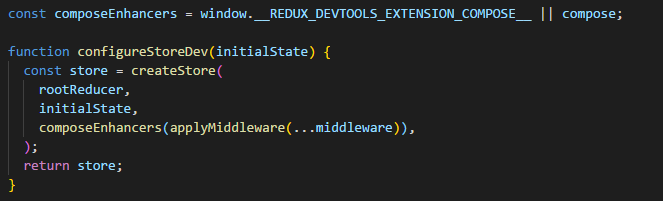
\includegraphics[width=14cm]{img/redux-devtools}\\[0.5cm]
	\end{center}
\end{figure}

Enkel het hoofdproject wordt geconnecteerd met de redux-devtools extension. Als dus gekeken wordt naar de state tree, dan is dit deze van het hoofdproject. Wanneer er meerdere projecten met elkaar gecombineerd worden, zal er nog steeds enkel de state tree van de hoofdapplicatie staan. Het zou dan ook een absolute meerwaarde zijn om deze debug tool te kunnen gebruiken met de gecombineerde state tree van beide projecten.
\autocite{devtools}

Er werd ook onderzocht of er meerdere stores mogelijk zijn voor gebruik, dan zou er per geïntegreerd project een nieuwe store bijkomen in het hoofdproject.
Het originele Flux patroon beschrijft meerdere stores in één applicatie, elke store houdt een verschillend segment van domein data vast. Dit kan problemen veroorzaken zoals een store die geforceerd wordt om te wachten op een andere store die nog geüpdatet moet worden. Dit is niet noodzakelijk zo in Redux, omdat de splitsing tussen data domeinen al bekomen wordt door het splitsen van één enkele reducer in een reeks kleinere reducers.

Het is mogelijk om meerdere verschillende Redux stores in een applicatie te hebben, maar het voorgenomen patroon bevat slechts één store. Met één store wordt het mogelijk om Redux devtools te gebruiken, het maakt persisteren van data simpeler alsook de subscription logica. Er zijn echter een aantal geldige redenen om meerdere stores te gebruiken in Redux:
\begin{itemize}
	\item Het oplossen van een performantieprobleem dat veroorzaakt wordt door het te veel updaten van een deel van de state.
	\item Het isoleren van een Redux applicatie als een component in een grotere applicatie, in dit geval is het aan te raden een store te creëren per root instantie.
\end{itemize}
Nieuwe stores aanmaken is niet het eerste waar naar gekeken moet worden, het is beter om reducer compositie toe te passen en enkel meerdere stores te gebruiken als het probleem niet opgelost kan worden op deze manier.

Gelijkaardig is het mogelijk om de store instantie aan te spreken door deze rechtstreeks te importeren, dit is eveneens geen aan te raden patroon in Redux. Wanneer een instantie van de store wordt gemaakt en geëxporteerd uit de module, dan wordt deze een singleton. Dit wil zeggen dat het moeilijker wordt om een Redux applicatie als een component van een grotere applicatie te isoleren. Er kan dan ook geen server rendering geactiveerd worden, want op de server worden er verschillende store instanties gecreëerd voor elke request die gemaakt wordt.

Het is best practice om de root component te wrappen in een <Provider> en dan gaat React Redux zorgen dat de store doorgegeven wordt naar beneden. Op deze manier moeten components geen store module importeren en worden de isolatie van een Redux app of het activeren van server rendering veel makkelijker om te implementeren.
\autocite{Redux02}

Dit staat ook beschreven in een provider patroon volgens \textcite{provider}. Veel React libraries moeten hun data doorgeven doorheen de component tree. Bijvoorbeeld, Redux moet zijn store doorgeven en React Router moet de huidige locatie doorgeven. Dit zou kunnen opgelost worden door een gedeelde, muteerbare state. Dit werkt enkel als er één state is. Wanneer er geprerenderd wordt op de server is het onmogelijk om te vertrouwen op deze implementatie. Gelukkig zorgt React voor een manier om de data van boven naar beneden te krijgen: \textit{context}. Dit kan aanzien worden als het globale object van de component tree.

Helemaal bovenaan in de app moet er dus een provider zijn. De enige rol die deze provider zal hebben is het toevoegen van gewenste data aan de context van de tree zodat alle afstammelingen ook toegang hebben tot deze data.


\paragraph{Connectie met React}
React bindings zitten echter niet standaard in Redux, eerst moet de npm-package react-redux worden geïnstalleerd. Om React en Redux samen te laten functioneren wordt gebruik gemaakt van een opsplitsing in presentationele en container components. (zie figuur 1.4 uit de lijst van figuren) 

\begin{figure}
	\begin{center}
		\caption{Verschillen tussen presentationele en container components. Verkregen van \textcite{prescon}}
		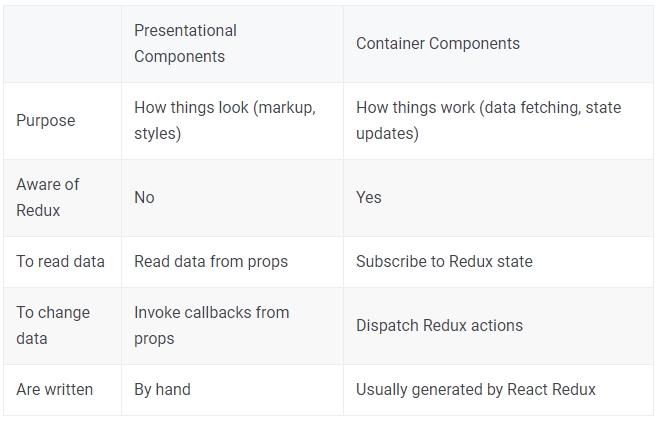
\includegraphics[width=13cm]{img/presentational-vs-container}\\[0.5cm]
	\end{center}
\end{figure}

Presentationele components zijn -zoals de naam aangeeft- prioritair voor de visualisatie. Ze verkrijgen enkel data via de props en sturen geen actions aan. 

Daar waar presentationele components gericht zijn op de visualisatie, zijn de container components gericht op het functionele aspect. Ze voorzien andere container (of presentationele) components van data en gedrag. Deze components gaan ook actions aanroepen om aan te duiden dat de data moet veranderen.  
\autocite{prescon}
\autocite{prescon2}

\subparagraph{Containers}
Het idee achter containers is dat ze de data gaan ophalen en dan de corresponderende sub-component gaan renderen. Deze data wordt gehaald uit de state en omgezet naar props voor die container. Daarna krijgen de sub-componenten de juiste props mee om hun data te renderen. 
\autocite{containercomp}

\section{Middleware}
In het Redux framework is middleware de code die zich bevindt tussen het krijgen van een request en het verzenden van een response. Express bijvoorbeeld kan CORS headers (mechanisme dat extra HTTP headers gebruikt om te laten weten aan de browser dat een web applicatie met een bepaalde oorsprong gemachtigd is om resources te gebruiken van een server met een verschillende oorsprong), logging, compressie,… toevoegen. De beste voorziening van middleware is dat het chainable is, er kan gebruik gemaakt worden van meerdere onafhankelijke third-party middleware in een enkel project.
 
Redux middleware gaat andere problemen oplossen dan de Express middleware, maar het is conceptueel dezelfde manier. Redux middleware gaat een third-party extension point voorzien tussen het dispatchen van een action en het moment dat deze action een reducer bereikt. Redux middleware wordt voornamelijk gebruikt om te loggen, voor crash reports, routing,…

Één van de voordelen van Redux is dat de veranderingen van de state voorspelbaar en transparant zijn. Elke keer een action gedispatched wordt, zal de nieuwe state berekend en opgeslagen worden. De state kan niet veranderd worden door zichzelf, maar enkel ten gevolge van een specifieke action. Via middleware is het mogelijk om elke action die verzonden wordt in de app te loggen samen met de state die erna verkregen wordt. Wanneer iets mis gaat kan er dan makkelijk teruggekeken worden in de log en kan er snel gezien worden welke action de state corrupt heeft gemaakt. De meest naïeve oplossing is om zelf de action en de volgende state te loggen elke keer de dispatch functie van de store wordt opgeroepen. Een betere oplossing is om de dispatch functie te vervangen. Met behulp van middleware kan zelf een logger geschreven worden die dan later enkel toegevoegd moet worden aan de store van de applicatie. Middleware wordt op dezelfde manier toegevoegd aan de store als de Redux devtools extension. Waar voor de Redux devtools extension een extra parameter wordt toegevoegd zal voor de middleware ook een parameter worden toegevoegd die meerdere middleware kan bevatten. 
\autocite{Redux02}

Om een betere verstandhouding van Redux te krijgen werd ook naar de voorgangers van Redux gekeken, waaronder Flux. Hieronder worden de verschillen en de gelijkenissen tussen Flux en Redux overlopen. 
Het eerste verschil is dat Flux een patroon is en Redux een library. Flux is een mooiere naam voor het observer patroon dat wat aangepast is voor React. Facebook heeft echter ook een aantal tools ontwikkeld die helpen in de implementatie van het Flux patroon. 

Flux en Redux hebben beide actions. Deze Actions kunnen vergeleken worden met events. In Flux is een action een simpel JavaScript object en dat is in het standaard geval ook zo in Redux. Wanneer er gebruik gemaakt wordt van Redux middleware kan het echter zo zijn dat actions ook functies en promises kunnen zijn. 

Met Flux is het de conventie dat er meerdere stores per applicatie zijn waarbij elke store een singleton object is. In Redux is het de conventie dat er maar één store per applicatie is. 

Flux heeft een enkele dispatcher en alle actions moeten door deze dispatcher gaan, dit is eveneens een singleton object. Een Flux applicatie kan geen meerdere dispatchers hebben. Dit is nodig omdat een Flux applicatie meerdere stores kan hebben en de afhankelijkheden tussen deze stores hebben een manager nodig, de dispatcher. In Redux is er geen dispatcher entiteit. In plaats daarvan heeft de store een dispatch proces van zichzelf. Een Redux store heeft een aantal simpele API functies, één daarvan is het dispatchen van actions.

De logica van wat er moet gebeuren wanneer er een action ontvangen wordt, zit in de store zelf bij Flux. De store heeft ook de flexibiliteit om te kiezen welke stukken data deze publiekelijk toegankelijk wil maken. Het slimste object in Flux is de store. In Redux zit de logica dan in de reducer. Een store kan niet gedefinieerd worden zonder reducer functie. Hier is het slimste object de reducer. Redux gaat ook gewoon alle data beschikbaar maken die geretourneerd wordt van de reducer. 

Nog een groot verschil is dat de state immutable is in Redux. Dit wordt makkelijk bekomen door van de reducers pure functies te maken. In Flux is hier geen restrictie, de state kan gemuteerd worden zoals gewenst.
\autocite{flux}

\section{Npm}
Om de twee projecten met elkaar te laten communiceren, wordt gebruik gemaakt van npm. De extensie op Redux zal geschreven worden en onder een eigen package gepubliceerd worden op npm, op deze manier kan de geschreven extensie aangesproken worden. 

Npm is 's werelds grootste software register met ongeveer 3 biljoen downloads per week. Het register bevat meer dan 600.000 packages. Open source developers van elk continent gebruiken npm voor het delen en lenen van packages. Veel organisaties gebruiken npm ook voor privaat development, zoals in dit onderzoek ook het geval is. 

Npm bestaat uit 3 verschillende componenten.
\begin{itemize}
	\item de website
	\item de Command Line Interface (CLI)
	\item het register
	
\end{itemize}

De website wordt gebruikt om verschillende packages te zoeken of om zelf packages op te publiceren, privaat of publiek. Deze publicatie kan via de CLI gedaan worden.

De grootste reden om npm te gebruiken is om bestaande packages aan te passen en te specialiseren naar eigen apps. Natuurlijk kan ook gebruik gemaakt worden van bestaande custom packages van andere gebruikers.
\autocite{npm}

\section{Webpack}
De meeste React-Redux projecten maken gebruik van Webpack. Webpack heeft veel populariteit gewonnen door het gebruik in React. Webpack is een statische bundelaar van modules voor JavaScript applicaties. Het kleinste project dat gebundeld kan worden met webpack bestaat uit een input en een output. Wanneer webpack bezig is met het verwerken van de applicatie, maakt het intern een \textit{dependency graph} aan. Deze wordt geconstrueerd door alle imports af te lopen. Het bundelen van modules begint bij de door gebruiker gedefinieerde entries.
\begin{description}
	\item[Een entry point] 
	 gaat aanduiden welke module webpack het eerst moet beginnen builden vanuit zijn interne dependency graph. Webpack gaat dan kijken van welke andere modules en libraries dit entry point afhankelijk is (direct en indirect). 
\end{description}

Standaard is dit entry point de index file, maar deze kan uiteraard veranderd worden of er kunnen zelfs meerdere entry points toegevoegd worden. Samen met de entry point(s) wordt meestal ook de output property gedefinieerd. Via deze property weet webpack naar waar de bundels verzonden moeten worden en hoe deze moeten heten. De standaardsetting hiervoor is de dist folder.

In de meeste applicaties zitten er echter niet enkel JavaScript files. Soms worden image imports gedaan of wordt er via een url gewerkt. Webpack verstaat echter enkel JavaScript files. Om het mogelijk te maken om andere bestandtypes te converteren in geldige modules moeten loaders toegevoegd worden. Deze modules kunnen dan gebruikt worden door de applicatie en toegevoegd worden aan de dependency graph.
\autocite{webpack} 

\begin{description}
	\item[Een loader] heeft een \textit{test} en een \textit{use} property. De test property geeft weer welke file of files die er getransformeerd moeten worden. Een use property toont aan welke loader gebruikt moet worden voor deze transformatie.
\end{description}

Loaders worden gedefinieerd in de \textit{rules} property.
Waar loaders worden gebruikt voor de transformatie van bepaalde modules, zorgen plugins ervoor dat de bundle geoptimaliseerd wordt. Plugins gaan altijd vooraf aan een require statement en kunnen later aangepast worden door extra opties toe te voegen. 


%%=============================================================================
%% Methodologie
%%=============================================================================

\chapter{Methodologie}
\label{ch:methodologie}

%% TODO: Hoe ben je te werk gegaan? Verdeel je onderzoek in grote fasen, en
%% licht in elke fase toe welke stappen je gevolgd hebt. Verantwoord waarom je
%% op deze manier te werk gegaan bent. Je moet kunnen aantonen dat je de best
%% mogelijke manier toegepast hebt om een antwoord te vinden op de
%% onderzoeksvraag.

\section{Analyse}
Eerst werd een denk-analyse uitgevoerd om te achterhalen welke manieren er waren om de twee projecten met elkaar te laten communiceren.

Aangezien er aanpassingen moesten gebeuren aan het Scratch project omdat een rechtstreekse import niet werkte door het gebrek aan functionaliteit, werd geopteerd voor een nieuwe versie van het Scratch project te maken en deze te publiceren op npm. 

Om deze analyse verder uit te voeren werd gekeken naar wat de store van het hoofdproject nodig had als parameters. Daarna werden een reeks methodes uitgeprobeerd om te zien wat wel werkte en wat niet.


\section{Methodes}
\subsection{Functie combineReducers}
In de eerste methode werd geprobeerd om de root reducer van het scratch project rechtstreeks te integreren in de store van het hoofdproject. In de configuratie van de store wordt meegegeven wat de root reducer is en wat de initiële state van de applicatie is. De bedoeling was om een grote gecombineerde root reducer te maken om daarmee de store te initialiseren. Het enige wat hier aangepast werd aan de scratch-integration package was het exporteren van de root reducer in de index file.

Twee root reducers met elkaar combineren via de methode \textit{combineReducers} gaat echter niet zomaar. Deze methode is een functie met als parameter de reducers die moeten gecombineerd worden. Zoals eerder vermeld bevat een reducer een key en een value. De parameter bevat dus een lijst van reducers met elk hun key en value. De functie \textit{combineReducers} overloopt deze lijst en vraagt eerst alle keys op en schrijft deze weg in een nieuwe variabele. Daarna wordt voor elke reducer key gekeken als de corresponderende value een functie is. Als dit zo is, dan wordt deze reducer weggeschreven in een nieuwe lijst variabele.   

Deze functie retourneert dan opnieuw een functie 'combination'. In de scope van deze functie zitten onderandere twee lijsten. Een lijst voor de finale reducer keys en een lijst voor de finale reducers. 
 
Omdat deze na combinatie in de scope van de functie zitten, is het onmogelijk om na een eerste combinatie een tweede combinatie uit te voeren. Dit zorgt er dus voor dat eenmaal er een root reducer gecombineerd is, deze niet opnieuw kan gebruikt worden om nog eens te combineren met een andere root reducer. Om hier verder op in te spelen werd naar een tweede methode gezocht. 

\subsection{Object export}
Als tweede methode werd geprobeerd om geen rechtstreeks gebruik te maken van de root reducer van Scratch, maar om alle reducers te combineren in een groot object en dan dat object exporteren. Om deze methode mogelijk te maken moet de root reducer van het hoofdproject ook een object zijn en geen gecombineerde functie. Anders keert het probleem van de function scope terug. Met beide root reducers als object is het wel mogelijk om een gecombineerde root reducer af te leveren. De lijsten van de reducer keys en reducers bevatten dan de keys en reducers van beide projecten. Hierdoor wordt dus de volledige functionaliteit omvat van beide projecten.

\subsubsection{Nadelen}
Een eerste nadeel van deze methode is dat er dan ook met de root reducer van het hoofdproject rekening moet gehouden worden. Deze mag dan namelijk ook niet gecombineerd zijn. Om deze methode uit te voeren was er een gedeeltelijke herstructurering nodig, waardoor deze methode eigenlijk al niet meer optimaal is. 

Een tweede nadeel zijn de veranderingen in het Scratch project. Stel dat er een reducer bijkomt of verwijderd wordt, dan moet dit altijd manueel aangepast worden vooraleer er terug een werkende versie geproduceerd wordt. Indien er enkel nood is aan de root reducer die geëxporteerd wordt, dan zou dit geen probleem zijn aangezien deze veranderingen mee opgenomen worden in de combinatie van de root reducer. Door elke reducer afzonderlijk in een nieuw object te steken en zo te exporteren wordt er heel wat extra onderhoudswerk gecreeërd voor deze package.  

Een derde nadeel zijn de configuraties en dependencies die nodig zijn om het Scratch project te laten draaien. 
Elke dependency die gebruikt wordt, moet ook mee overgenomen worden in de package.json van het hoofdproject. Dit zorgt er ook voor dat de configuraties van webpack ook moeten meegenomen worden. Om dit te realiseren werd een nieuwe package gemaakt van de bestaande react-scripts package met de uitbreidingen die nodig zijn om een succesvolle integratie te verkrijgen.

\subsection{Eigen methode}
Als laatste methode werd gezocht naar een alternatief voor het vele onderhoudswerk die zich voordoet bij een object export. De bedoeling van deze extensie zou als het ware een uncombineReducers methode zijn. Op deze manier kan snel alles los gemaakt worden van elkaar om dan later opnieuw te kunnen combineren. Op deze manier kan een lineaire structuur verkregen worden. Momenteel is het niet mogelijk om van reeds gecombineerde root reducers een nieuwe reducer te combineren met een lineaire structuur in plaats van een geneste structuur. 

\paragraph{Analyse}
Om een extensie te schrijven is eerst een duidelijk inzicht nodig in de methode combineReducers. Hiervoor werd dus eerst een analyse gedaan van deze methode. 

De methode neemt reducers als parameter. Er worden eerst twee lokale variabelen gemaakt, de reducerKeys met daarin de keys van de reducers die als parameter werden meegegeven en de finalReducers. Daarna wordt -zolang er reducerKeys zijn- de juiste reducer opgehaald aan de hand van zijn key en wordt er gekeken als het type een functie is of niet. Als het inderdaad een functie is dan zal deze worden opgeslaan in de finalReducers.

Nu kan er een nieuwe variabele finalReducerKeys aangemaakt worden met daarin de keys van de finalReducers. Daarna wordt er een functie geretourneerd met dezelfde syntax als de reducer (state en action). Er wordt opnieuw per key overlopen, deze keer om een object te verkrijgen via \textit{reduce} aan de hand van de state voor deze key.

\paragraph{Werkwijze}

Er werd getracht om van een root reducer, die reeds gecombineerd is, de reducer keys aan te spreken van zijn onderliggende reducers. Dit bleek echter niet mogelijk omdat deze vastzitten in de function scope van combineReducers. Indien dit mogelijk was, kon op deze manier een lineaire combinatie gemaakt worden van meerdere root reducers.


 






% Voeg hier je eigen hoofdstukken toe die de ``corpus'' van je bachelorproef
% vormen. De structuur en titels hangen af van je eigen onderzoek. Je kan bv.
% elke fase in je onderzoek in een apart hoofdstuk bespreken.

%\input{...}
%\input{...}
%...

%%=============================================================================
%% Conclusie
%%=============================================================================

\chapter{Conclusie}
\label{ch:conclusie}

%% TODO: Trek een duidelijke conclusie, in de vorm van een antwoord op de
%% onderzoeksvra(a)g(en). Wat was jouw bijdrage aan het onderzoeksdomein en
%% hoe biedt dit meerwaarde aan het vakgebied/doelgroep? Reflecteer kritisch
%% over het resultaat. Had je deze uitkomst verwacht? Zijn er zaken die nog
%% niet duidelijk zijn? Heeft het onderzoek geleid tot nieuwe vragen die
%% uitnodigen tot verder onderzoek?

\section{Inleiding}
Redux is een framework die nog maar 3 jaar bestaat. Er is wel al veel documentatie beschikbaar en veel problemen zijn reeds ontdekt en opgelost, maar zeker niet alles staat beschreven. 

Bijvoorbeeld hoe 2 React-Redux projecten met elkaar kunnen interageren staat nergens beschreven. Omdat hier geen best practices vermeld werden, is de keuze gemaakt om via npm packages te werken. Op deze manier kan het ene project snel geïntegreerd worden in het andere. 

Het was echter niet voldoende om deze package gewoon te installeren. Wanneer dan een component werd aangeropen zou de state niet volledig zijn. De state bevat dan enkel objecten van het hoofdproject en niet van het geïntegreerde project. Om deze reden moeten de reducers geëxporteerd worden uit het geïntegreerde project. 

\section{Performantie}
Zoals eerder vermeld was de oplossing om deze reducers in een object te steken en dit te exporteren. Het grootste probleem hierbij is dat veranderingen in het project dat geïntegreerd moet worden grote gevolgen kan hebben. Dit werd ondervonden door het open source project van Scratch. Na een update van Scratch uit en de bijhorende update om de package up to date te houden werkte deze niet meer. Dit kwam door een verandering in de structuur van de reducers, waardoor het niet meer de juiste reducers waren die geëxporteerd werden. Dit zorgt er dus voor dat er zeer aandachtig moet gebleven worden bij updates. Om deze reden zou er nood zijn aan een methode uncombineReducers of een alternatief waardoor er enkel met de root reducer rekening zou gehouden moeten worden. Dan zouden externe updates geen grote impact meer hebben en kan deze snel terug geïntegreerd worden.

Deze methode is niet optimaal, aangezien er heel wat onderhoudswerk bij komt kijken om de package up to date te houden. Een bijkomend probleem is dat met deze methode ook alle dependencies moeten overgenomen worden alsook de webpack configuraties. 

Deze methode wordt al een heel stuk performanter door het te integreren project te combineren in webpack, op deze manier is het niet meer nodig om alle dependencies toe te voegen aan het hoofdproject en wordt de package voor de webpack configuraties overbodig. 

Zoals eerder gezegd is deze methode afhankelijk van de veranderingen in het te integreren project. Als hier quasi geen veranderingen in moeten gebeuren zal dit geen grote impact hebben, als er constant veranderingen in gebeuren dan zal deze methode niet meer optimaal zijn. 

\section{Complexiteit}
Er zijn een aantal objectieve maatstaven die ontwikkeld zijn voor de complexiteit van software te meten. In grote lijnen kan men deze maatstaven verdelen in maten voor complexiteit die zijn gerelateerd aan de omvang van een software-programma, en in maten voor complexiteit die zijn gerelateerd aan de structuur van zo'n programma. De simpelste maat voor de omvang is het aantal regels programmacode: hoe meer regels, hoe groter de complexiteit. Een ernstig nadeel van deze simpele metriek is dat men het verschil in uitdrukkingskracht van de verschillende programmeertalen volledig verwaarloost.

Men maakt ook geen onderscheid naar soorten regels code. Er zijn echter eenvoudige regels code en er zijn complex samengestelde regels programmacode. Om hieraan tegemoet te komen, heeft Halstead een meer verfijnde metriek ontwikkeld. In zijn theorie is de complexiteit en de daarmee samenhangende programmeerinspanning afhankelijk van de omvang van een programma en van het niveau van structurering. Hoe groter de omvang, hoe hoger de programmeerinspanning. hoe hoger (compacter) het niveau van structurering, hoe lager de inspanning. Zowel omvang als niveau van structurering zijn functies van het aantal verschillende operatoren en operanden in een programma.
\autocite{complexiteit01}

Men kan nu deze metriek toepassen op het voorbeeld met de gemaakte package in deze studie. n1 staat voor het aantal verschillende operatoren, n2 staat voor het verschillende aantal operanden, N1 is het aantal operatoren en N2 is het aantal operanden. Met deze nummers kunnen een aantal metingen berekend worden:
\begin{itemize}
	\item Vocabulair van het programma: n = $n_1$ + $n_2$ = 3 + 23 = 27.
	\item Lengte van het programma: N = $N_1$ + $N_2$ = 27 + 43 = 70.
	\item Berekende lengte van het programma: $N_3$ = $n_1$ $log_{2}(n_1)$ + $n_2$ $log_{2}(n_2)$ = 4,7549 +  104,0419 = 108,7968.
	\item Volume: V = N * $log_{2}(n)$ = 70 * 4,7549 = 332,8422.
	\item Moeilijkheid: D = ($n_1$/2) * ($N_2/n_2$) = 1,5 * 1,8696 = 2,8043.
	\item Inspanning: E = D * V = 2,8043 * 332,8422 = 933,3894.
\end{itemize}
De meeteenheid inspanning kan vertaald worden naar codeertijd aan de hand van de volgende relatie: de tijd T = E/18 = 51,8550 seconden.
Halstead kan ook een schatting geven van het aantal errors die in de implementatie zitten door naar het aantal geleverde bugs te kijken: B = E\textsuperscript{2/3}/3000 = 0,1245.

Deze metriek werd toegepast op het exporteren van de reducers in de gepubliceerde package en de code die nodig is om alle reducers opnieuw te importeren in een hoofdproject. Er kan geconcludeerd worden dat het een snelle codeertijd heeft dat gepaard gaat met een laag aantal geleverde bugs.

Een andere manier om de complexiteit van software te meten is via de cyclomatische complexiteit. Deze metriek is een quantitatieve meting van het aantal lineair onafhankelijke paden in de code en werd ontwikkeld door McCabe. 
De cyclomatische complexiteit wordt gedefinieerd als M = E - N + 2P.\newline
Waarbij: 
\begin{itemize}
	\item E = het aantal randen, verbindingen in een diagram
	\item N = het aantal knooppunten in een diagram
	\item P = het aantal geconnecteerde componenten
\end{itemize}
\autocite{cyclomatic}

In dit geval gaat het om een lineaire structuur zoals gezien kan worden in de figuur. De geëxporteerde package bevat 23 verbindingen, 24 knooppunten en 1 geconnecteerde component. Hiermee kan de cyclomatische complexiteit bepaald worden door M = 23 - 24 + 2 = 1. Volgende figuur verkregen uit \textcite{complexitynumbers} geeft een overzicht weer van de complexiteit waarde en zijn overeenkomstige betekenis. 

Hieruit kan afgelezen worden dat een nummer hoger dan 40 niet getest kan worden en een hoge kost en inspanning heeft. Een waarde tussen de 20 en 40 wordt aanzien als heel complexe code met lage test mogelijkheden en eveneens een hoge kost en inspanning. Een complexiteitswaarde tussen de 10 en 20 duidt op complexe code met gemiddelde testbaarheid, kost en inspanning. Een waarde tussen de één en 10 betekent dat de code goed gestructureerd en geschreven is, met een hoge testbaarheid en een lage kost en inspanning. Aangezien de berekende cyclomatische complexiteit 1 bedraagt, kan de conclusie getrokken worden dat de code gestructureerd is, een lage kost en inspanning heeft en makkelijk getest kan worden.






\section{Eindconclusie}
Dit onderzoek is nog niet klaar, de basis is wel gelegd om verder onderzoek te doen naar een methode om de root reducers van beide projecten met elkaar te combineren zonder dat daar veel extra onderhoud aan te pas komt. Als uitkomst was wel verwacht dat er een soort uncombineReducers zou gemaakt worden, helaas was dit niet mogelijk door de implementatie van deze functie. Er is wel een alternatief gevonden om toch het probleem op te lossen. 

Achteraf gezien bleek het een goede keuze om voor het Scratch open source project te kiezen. Dit is een project dat nog steeds in development is en dat nu overschakelt op JavaScript, waardoor het zeer interessant wordt om dit te kunnen integreren in een eigen applicatie.   

Dit is een belangrijk onderzoek omdat er nog geen soortgelijke onderzoeken zijn gedaan of gedocumenteerd werden.
Er zijn een aantal statistieken gevonden die duidelijk maken dat het een probleemstelling is die uitnodigt tot verder onderzoek. De npm package die de reducer exports verzorgde is opgericht eind februari. Dan werd gezocht naar hoe het mogelijk wordt om dit project snel integreerbaar te maken, waar tot een tijdelijke oplossing is gekomen begin maart. Deze package werd sinds dan ruim 7000 keer gedownload (figuur 9) met piekmomenten van 2168 downloads per week (figuur 8) en 946 downloads per dag (figuur 7) in maart. Door tijdsgebrek was het echter onmogelijk om deze package constant up to date te houden. Eind maart kan er nog een update gezien worden door het stijgende aantal downloads, wat duidt op het feit dat er wel vraag naar is.

%%=============================================================================
%% Bijlagen
%%=============================================================================

\appendix

%%---------- Onderzoeksvoorstel -----------------------------------------------

\chapter{Onderzoeksvoorstel}

Het onderwerp van deze bachelorproef is gebaseerd op een onderzoeksvoorstel dat vooraf werd beoordeeld door de promotor. Dat voorstel is opgenomen in deze bijlage.

% Verwijzing naar het bestand met de inhoud van het onderzoeksvoorstel

\section{Introductie} % The \section*{} command stops section numbering
\label{sec:introductie}
Vooraleer er dieper op het probleem kan worden ingegaan is er meer context nodig rond een aantal basisbegrippen van React en Redux.
Volgens de website van \textcite{Redux02}
React is een JavaScript library. Met behulp van React worden views gecreëerd voor elke state in onze applicatie. 
Redux is een state container voor JavaScript apps. Redux helpt om de afgebeelde data te beheren en beschrijft hoe er gereageerd wordt op user actions.  
Een store is een object die de volledige state-tree van de applicatie bevat. De enige manier om een state te veranderen in de store is door een action te dispatchen.
Een action zal er eigenlijk voor zorgen dat er data van de applicatie verzonden wordt naar de store. Dit is tevens de enige vorm van input voor de store. Actions beschrijven dus het feit dat er iets gebeurd is, maar ze beschrijven niet hoe de state van de applicatie verandert. Dit is de taak van een reducer, deze toont aan hoe de state veranderd is ten gevolge van een action die verzonden werd naar de store. Een container is dan weer verantwoordelijk voor het verkrijgen van data. Om die data te verkrijgen wordt er gebruik gemaakt van de connect functie (voor de store) en een functie die de data uit de state neemt en deze mapt naar zijn eigen props. Een container is ook verantwoordelijk voor het dispatchen van actions.  
Het probleem zit bij het samenvoegen van 2 react-redux apps tot 1 app. Er is geen manier bekend om beide stores te behouden in 1 project. Dit is relevant omdat er toch een aantal hits op Stack Overflow te vinden zijn voor dit probleem. 
2 React projecten die elk afzonderlijk een Redux store gebruiken kunnen als ze samengevoegd worden momenteel maar de volledige functionaliteit van 1 store gebruiken.  
Onderzoeksvraag: 


\begin{itemize}
	\item Op welke manier kunnen de stores van 2 react-redux apps onafhankelijk functioneren in 1 app? 
	
\end{itemize}



%---------- Stand van zaken ---------------------------------------------------

\section{State-of-the-art}
\label{sec:state-of-the-art}

Zoals eerder vermeld is er zeer weinig documentatie te vinden over dit probleem. Er zijn wel een aantal vragen in die richting op Stack Overflow gesteld. De antwoorden die op deze vragen gegeven zijn, bieden geen oplossing op lange termijn of bieden geen schaalbaarheid/uitbreidbaarheid. Er zal veel tijd gestoken worden in het verdiepen van de GitHub repository van Redux, geschreven door \textcite{Redux01}. Er is wel documentatie te vinden over de Redux-store sharen in meerdere components binnen hetzelfde project. Hier staat een uitgewerkt voorbeeld van op Stack Overflow door \textcite{2017}. Het wordt echter onduidelijk wanneer we de Redux-store willen sharen tussen meerdere projecten.   


% Voor literatuurverwijzingen zijn er twee belangrijke commando's:
% \autocite{KEY} => (Auteur, jaartal) Gebruik dit als de naam van de auteur
%   geen onderdeel is van de zin.
% \textcite{KEY} => Auteur (jaartal)  Gebruik dit als de auteursnaam wel een
%   functie heeft in de zin (bv. ``Uit onderzoek door Doll & Hill (1954) bleek
%   ...'')


%---------- Methodologie ------------------------------------------------------
\section{Methodologie}
\label{sec:methodologie}
Er zal geprobeerd worden een uitbreiding te schrijven op de bestaande Redux library. Zoals eerder vermeld houdt een redux store eigenlijk de hele state-tree van de applicatie vast. De bedoeling van deze uitbreiding zal zijn om een draaiende app te hebben met 2 onafhankelijke stores van 2 projecten. Deze realisatie zal gebeuren door het ene project om te zetten naar een npm-package. Op deze manier kunnen geëxporteerde componenten makkelijk geïmporteerd worden in het andere project. Met de uitbreiding zal geprobeerd worden om een store toe te voegen aan het project, zonder dat de andere store daar enige invloed van ondervindt. Om dit te kunnen realiseren zal het react-redux patroon goed moeten bestudeerd worden. Daarbij kan ook naar Flux en MobX gekeken worden om eventuele analogieën door te trekken. In dit onderzoek zullen een aantal grafieken worden gemaakt met de gemiddelde rendertijd van verschillende oplossingen (met bv: nesting en reducers importeren). Anderszijds wordt er ook naar de lines of code gekeken. Een groot criteria hierbij is dan het dupliceren van code of het vervuilen van de applicatie door code toe te voegen die ze eigenlijk niet nodig zou moeten hebben. 



%---------- Verwachte resultaten ----------------------------------------------
\section{Verwachte resultaten}
\label{sec:verwachte_resultaten}

Zoals eerder aangegeven worden er een aantal oplossingen verwacht. Enerzijds kan een nesting van de stores een mogelijke oplossing bieden, maar de vraag is dan of alle functionaliteit wordt behouden. Door het schrijven van de uitbreiding kan de rendertijd hoger zijn dan normaal. Een andere oplossing is door de reducers van het ene project samen te voegen met de reducers van het andere project, waarbij een hoger aantal lines of code verwacht wordt.

%---------- Verwachte conclusies ----------------------------------------------
\section{Verwachte conclusies}
\label{sec:verwachte_conclusies}

Een verwachte conclusie bij nesting is dat mogelijks niet alle functionaliteit behouden wordt. Een kopie nemen van de reducers van het ene project is geen efficiënte oplossing en wel om deze reden: stel dat er een update gepushed wordt naar de npm-package dan zou men alle reducers opnieuw moeten kopiëren naar het andere project. Tevens vervuilt dit ook de hoofdapplicatie. 

%%---------- Andere bijlagen --------------------------------------------------
% TODO: Voeg hier eventuele andere bijlagen toe
%\input{...}

%%---------- Referentielijst --------------------------------------------------

\printbibliography[heading=bibintoc]
%\addcontentsline{toc}{chapter}{\textcolor{maincolor}{\IfLanguageName{dutch}{Bibliografie}{Bibliography}}}

\end{document}
